% Chapter 6

\chapter{Experimental Protocol} % Main chapter title

\label{Chapter6} % For referencing the chapter elsewhere, use \ref{Chapter1} 

\lhead{Chapter 6. \emph{Experimental Protocol}}

%----------------------------------------------------------------------------------------

% TODO Explain the choice of algorithms and tracks (explain 0 shape track for better comparison)

The experimental protocol was designed around the nine experimental requirements, presented in \ref{expreq} and corresponding to the four research hypotheses introduced in \ref{reshypo}. \\
When starting the project, I found out that the project plan I had introduced in \ref{propla} could not work: the reward function requirement (E1) cannot be done before the DQN implementation (E4) and the DDPG implementation (E6), because the reward function will depend on the controller's outputs. Furthermore, because the DQN controller outputs discrete actions and the DDPG controller outputs continuous actions, they would have different reward functions. I decided to start with the second experimental requirement E2 (implementing the wall following controller), then assess it (E3). I then implemented and trained the Deep Q-Network controller (E4), defining the reward function at the same time (E1). I did the same with the DDPG controller, and finished with the Sim2Real gap assessment (E8) and the overall conclusions (E9). \\
As explained in \ref{reshypo}, the DQN and DDPG controllers will be trained on the "RedBull Ring" racetrack from \cite{bosello} for requirements E4 and E6. The assessment of all three controllers in the simulator (wall follower, DQN and DDPG) is then done on the RedBull track as well as the Silverstone (Annex \ref{silverstone}) and Monaco (Annex \ref{monaco}) racetracks. \\
I chose those specific tracks for several reasons. Firstly, I thought The Red Bull Ring track to be a good training map, because it presents most of the challenges that the controller will encounter on other racetracks: a sharp turn (n°3 Remus, see Annex \ref{redbull}), wide turns (6,7) and two long straight lines, all of that on a very short circuit, which I think makes for good training data. The second track, Silverstone, is much longer, with very long curves and some chicanes, which represents a different challenge: many small adjustments in the long curves, and very fast adjustments for the chicanes. The Monaco track also represents a different challenge, with a lot of hairpins turns (5,6 and 16, see Annex \ref{monaco}). \\
After some consideration I decided to also assess the controllers (experimental requirements E3, E5, E7) on a fourth track (see Annex \ref{oval}). This track has a very simple oval shape, which makes it easy to reproduce in real life using flexible tubing; this would make the Sim2Real gap assessment (experimental requirement E8) much more meaningful, because the metrics introduced in \ref{eva} would actually be comparable on a whole lap of the track and not just on a small portion of it. I chose the proportions of the track myself, to make it as compact as possible, but with a sufficient track width.


\section{Deep Q-Network implementation}
The Deep Q-Network controller that will be used to obtain experimental results is largely based on the implementation from \cite{bosello}. I will first explain the architecture of the code, and then introduce the differences I've made to the original code. \\
The UML diagram of the final code is shown in Figure \ref{uml}:
\begin{figure}[H]
\centering
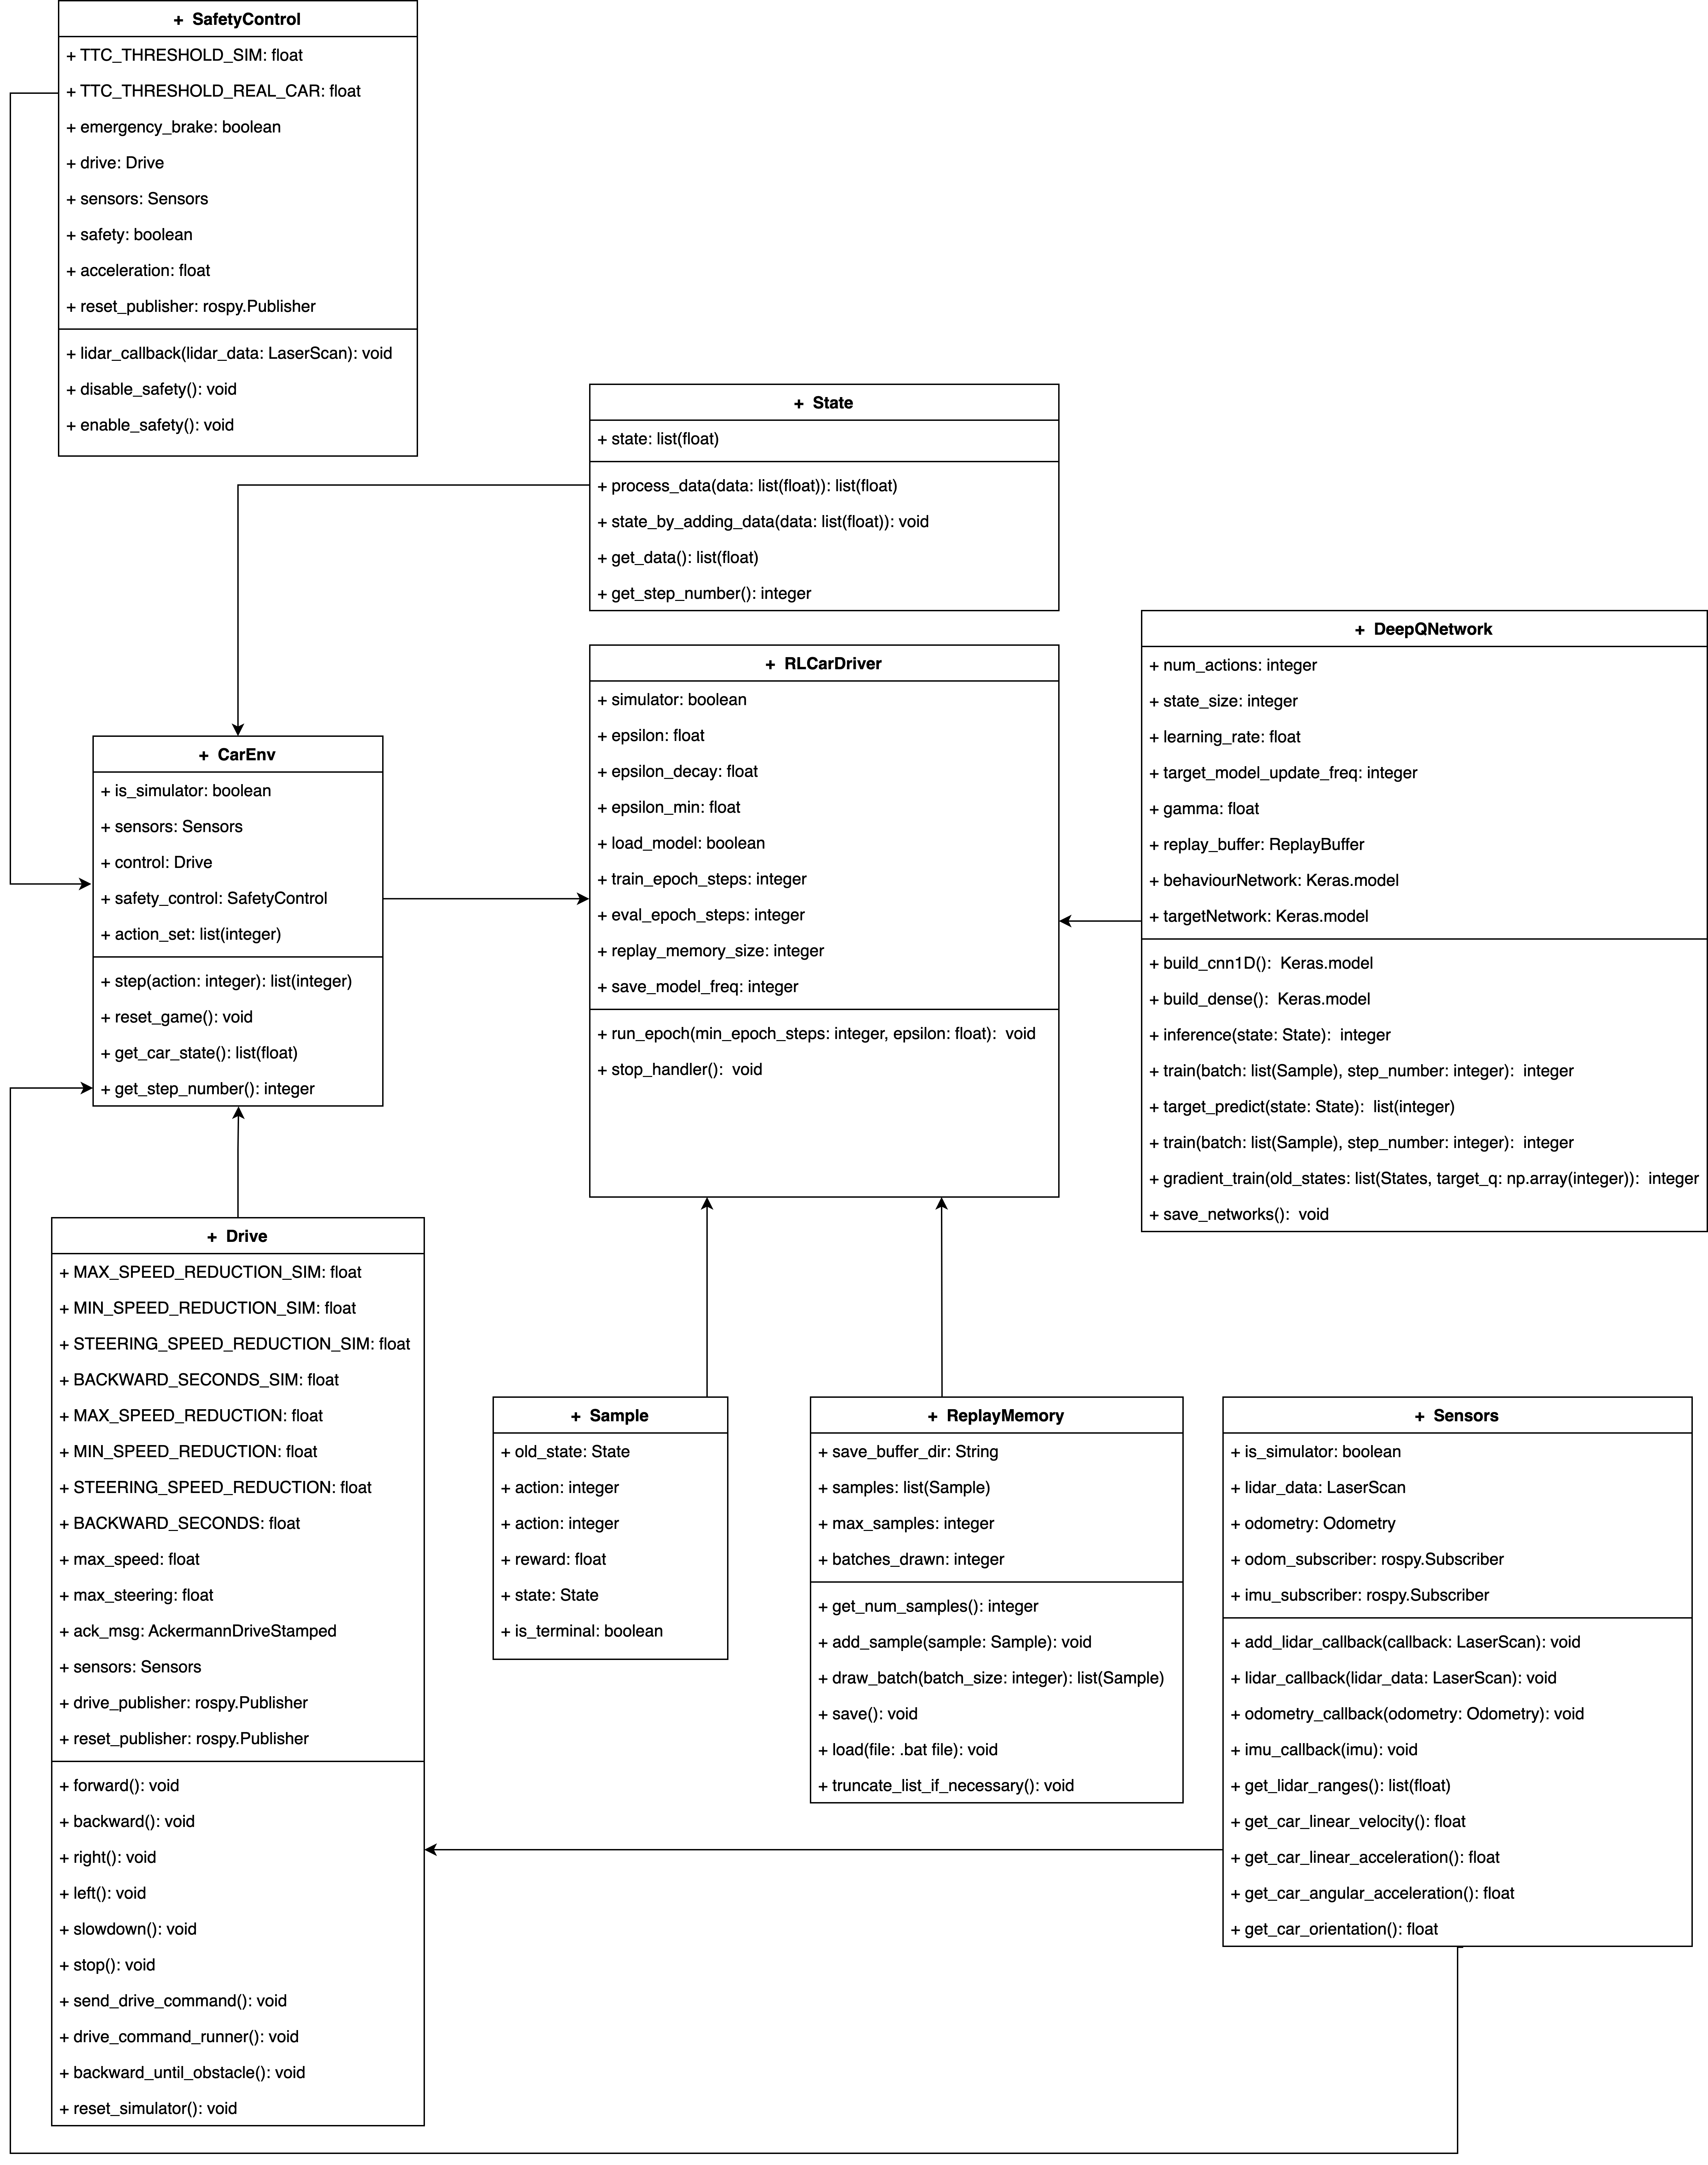
\includegraphics[scale=0.33]{Figures/UML_diagram.png}
\caption{UML diagram of the Deep Q-Network impementation (modified from \cite{bosello})}
\label{uml}
\end{figure}
The subscribers, publishers and topics are as shown in Figure \ref{pub_sub}:
\begin{figure}[H]
\centering
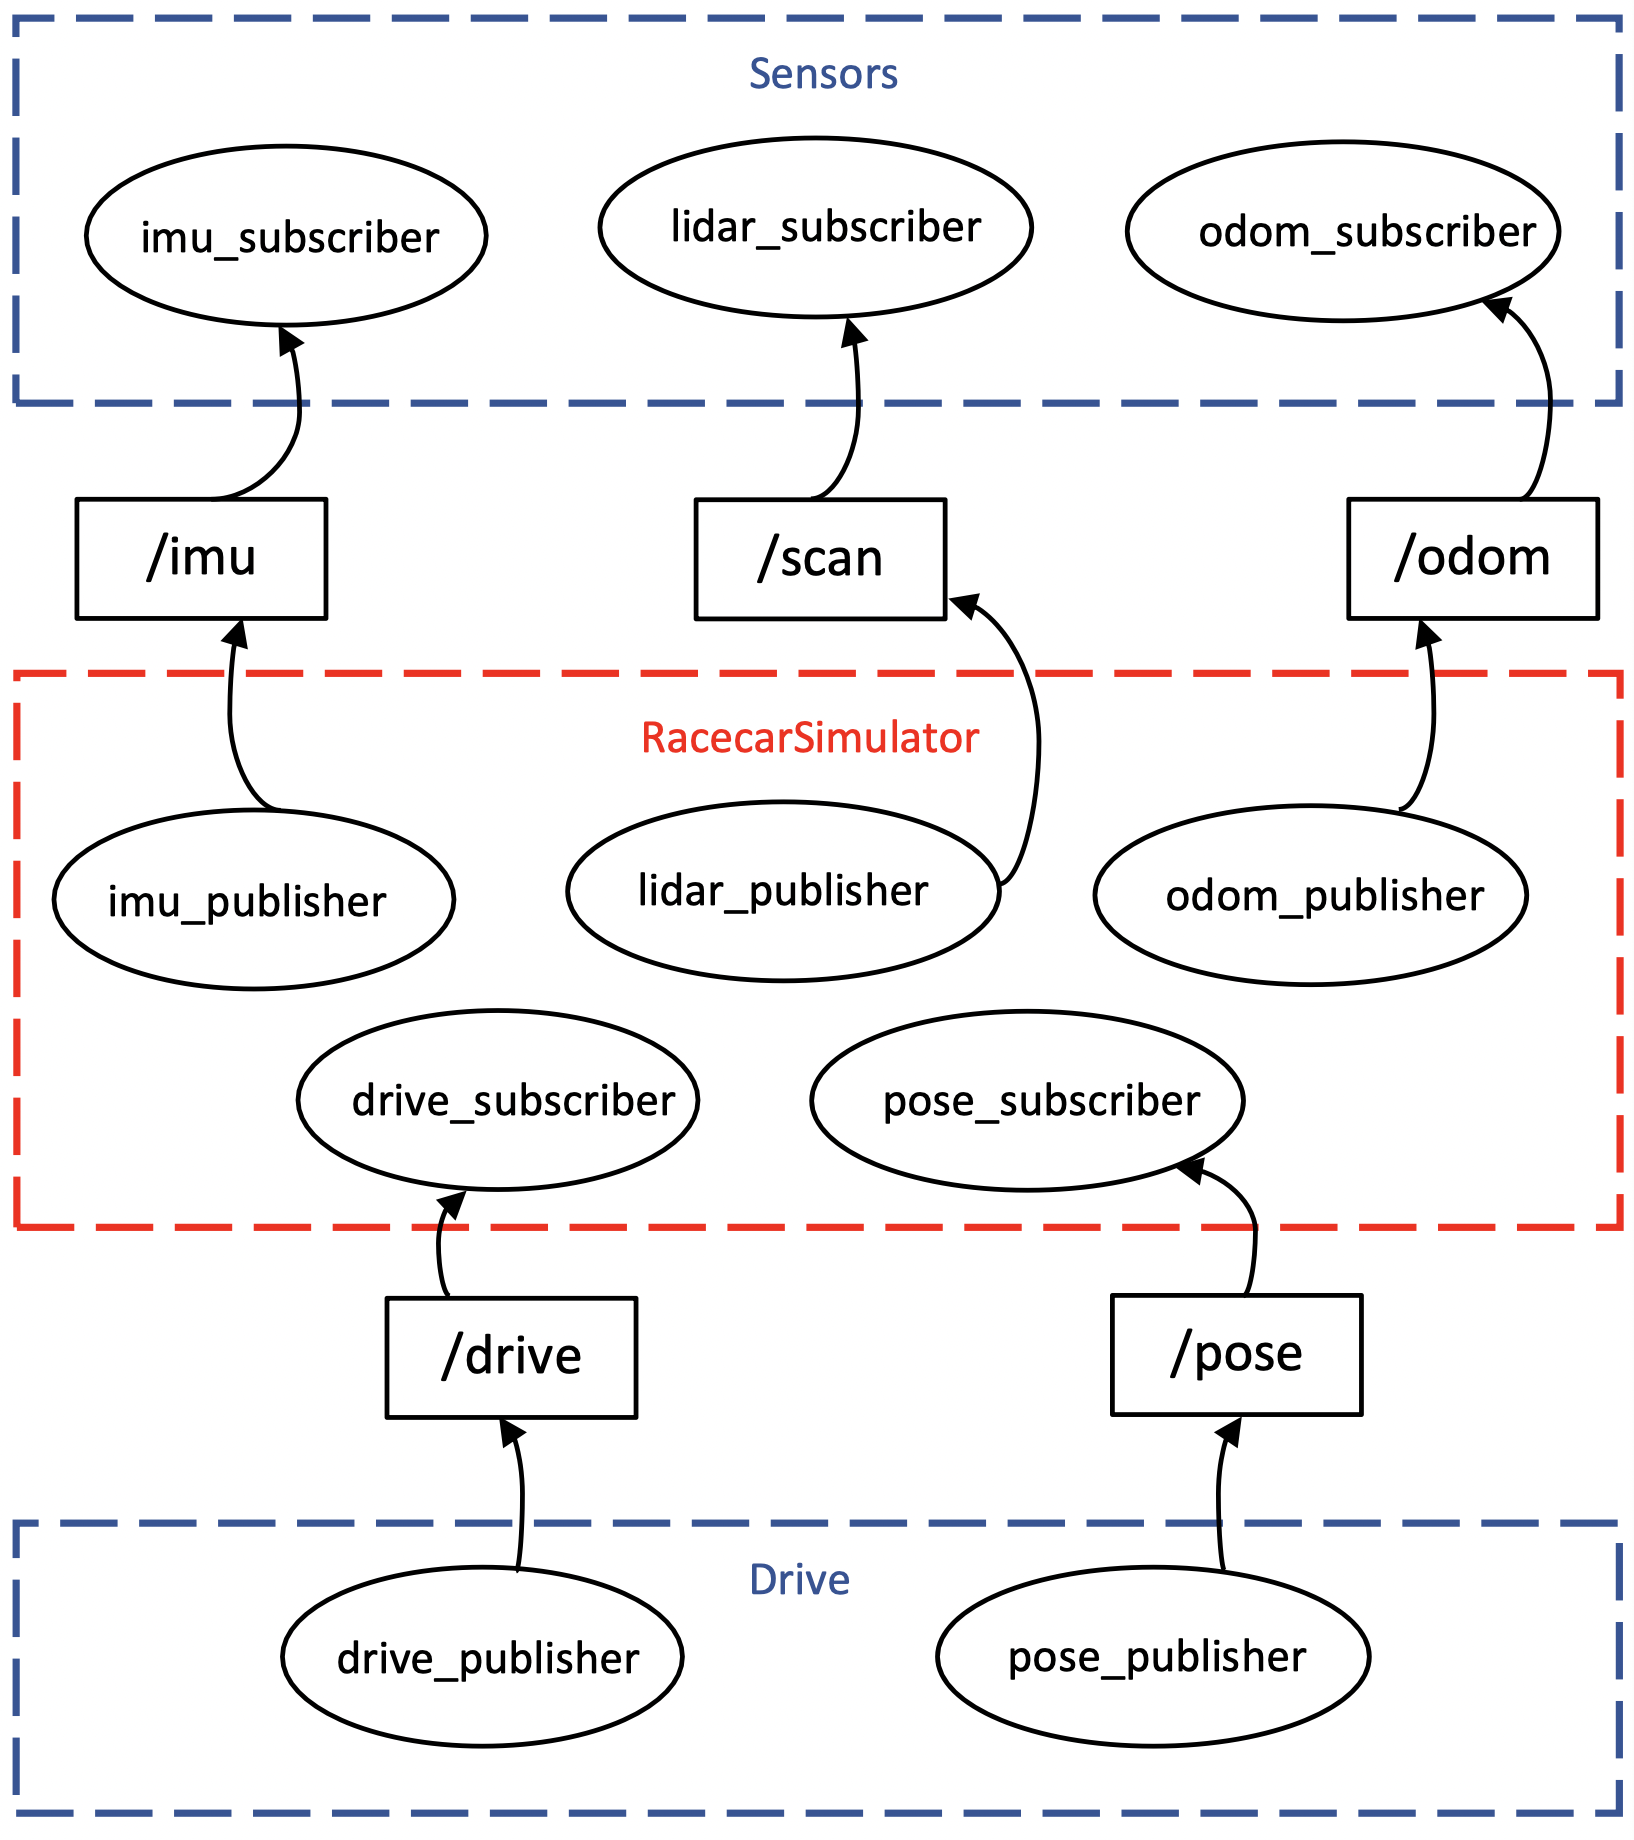
\includegraphics[scale=0.33]{Figures/pub_sub.png}
\caption{Subscribers, publishers and topics for the Deep Q-Network implementation}
\label{pub_sub}
\end{figure}
The agent drives as introduced in Figure \ref{inputs_outputs}. The data from the \verb|\odom| and \verb|\scan| topics is obtained through the \verb|get_car_state()| function, then is processed and stored in a state. The state stored in the replay memory is then fed to the \verb|behavior_predict(state)| function, which returns an array of 4 float values between 0 and 1, corresponding to each possible action. The action with the highest score is then sent to the \verb|step(action)| function, which calls the corresponding action function, for example \verb|forward()|. This action function then sends a desired speed and steering angle to the \verb|send_drive_command| function, which creates an Ackermann message. This message is finally published to the \verb|drive| topic by the \verb|drive_command_runner(ack_msg)| function.
\begin{figure}[H]
\centering
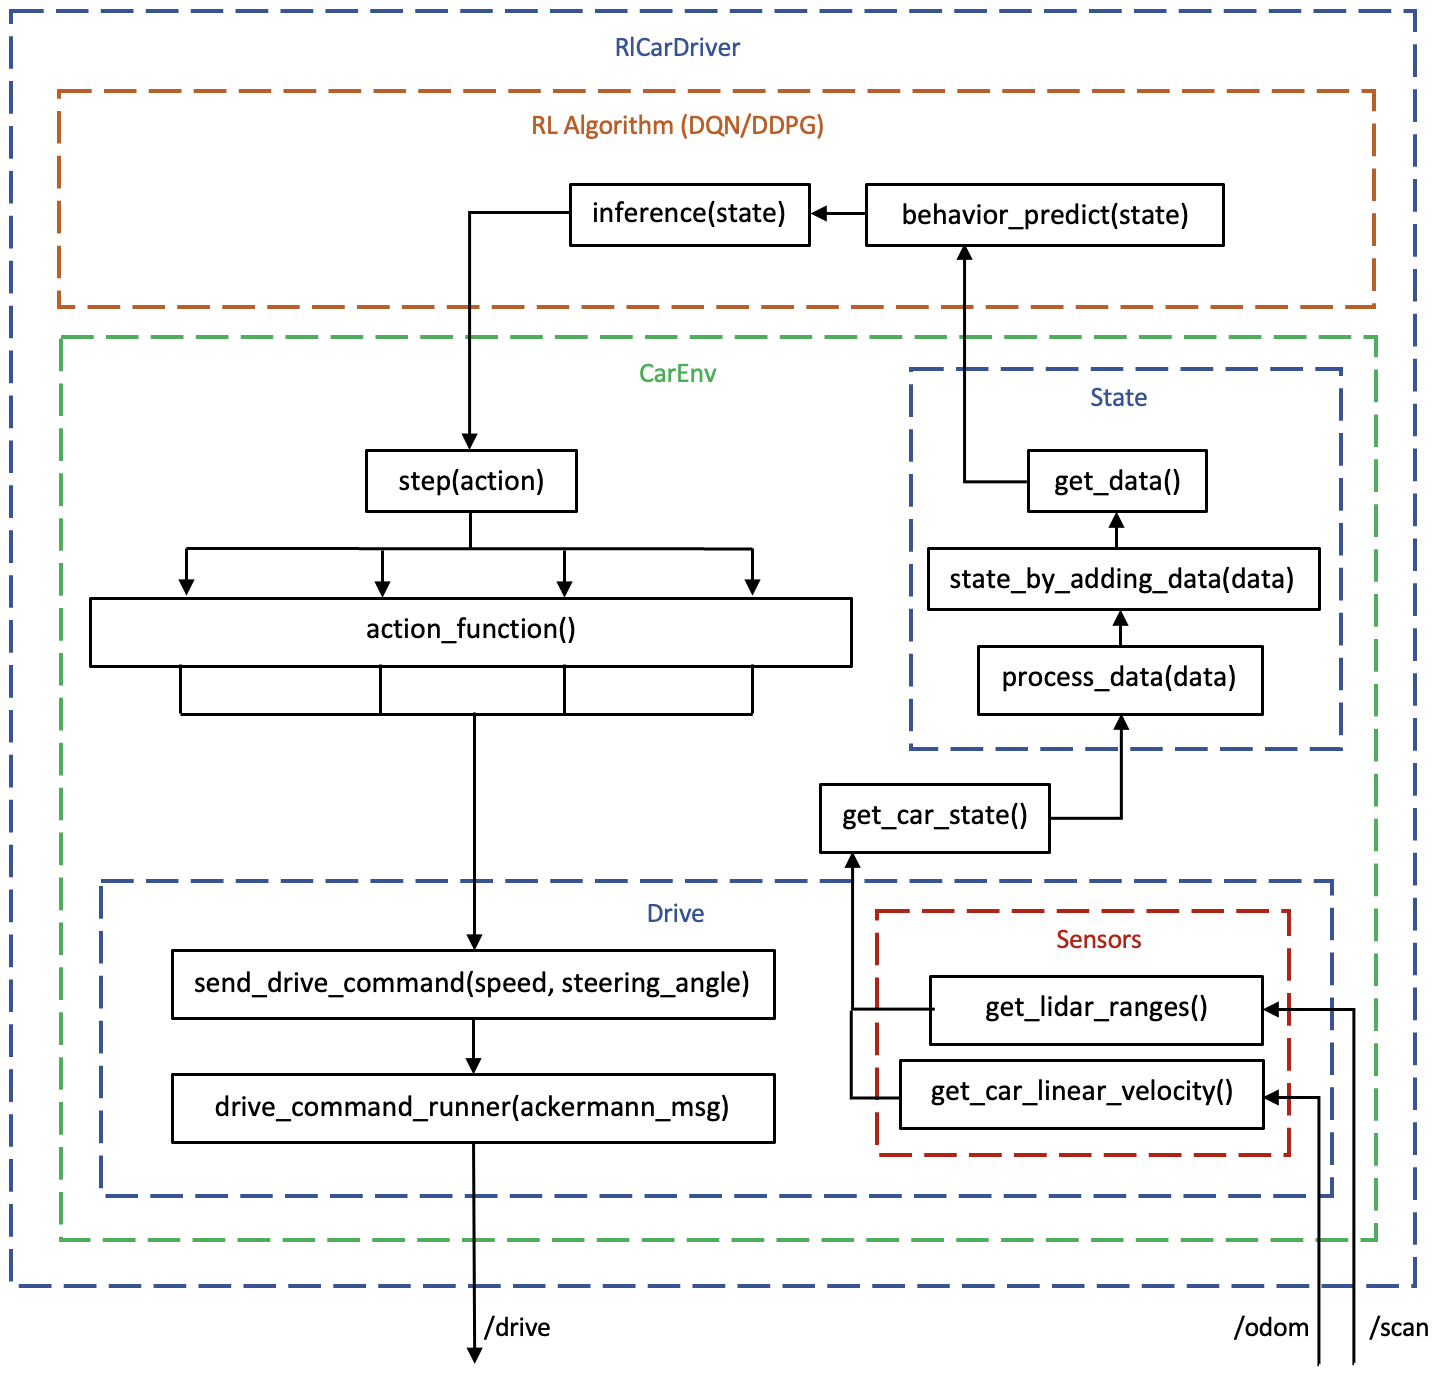
\includegraphics[scale=0.38]{Figures/inputs_outputs.png}
\caption{Functions involved in running an epoch and their inputs/outputs}
\label{inputs_outputs}
\end{figure}
The code is structured around three main classes: the \verb|RLCarDriver|, \verb|CarEnv| and \verb|DeepQNetwork| classes. \\
The \verb |RLCarDriver| class is responsible for three things: setting up the output and logging directory, parsing the parameters from user input and running the \verb |run_epoch()| function inside of a \verb |while(not stop)| loop. The \verb ||

\section{Reward functions}
The first requirement (E1), was to define a reward function which incentivises a safe, smooth and fast control of the car. A reward function has to be defined for both the DQN and the DDPG implementations. \\
Several reward functions were considered for the DQN controller. \\
Before defining the reward function, I had to define the actions that the RL agent would be able to perform. The controller can send two types of commands to the agent through an AckermannDrive Message: a desired forward speed command (m/s) and a desired steering angle command (radians). Thus, the reward function needs to incorporate at least one of those two variables. \\
The problem is that DQN can only output discrete actions, whereas the steering and speed outputs of the car are continuous. A simple solution is to discretise the action space, for example by replacing all the possible steering angles by just a few increments, and doing the same for speed. The car can steer from around -40° to +40°: with 4° increments this gives us 20 steering outputs; the car can go from 0 to 5 m/s, with 1 m/s increments this gives 5 possible speed outputs: this results in 100 possible outputs. The controller is now facing the ``curse of dimensionality" problem. There are much more states to explore, and the training time will increase dramatically. \\
To avoid this issue, I decided to instead limit the controller outputs to just 4: going forward at full speed, turning left or right at reduced speed and maximum steering angle, and keeping the same steering angle at reduced speed. \\
This way, the controller is less smooth but can learn faster; if necessary, it is easy to add a few other outputs (turning slightly left/right), with different steering angles and speeds. \\
The first attempt was to have a reward proportional to the speed of the car: for step $t$, $r(t) = v(t) \cdot \frac{1}{V_{max}}$. This resulted in a few oscillations and frequent collisions because the agent is not looking at the LiDAR data and thus rarely slows down. \\
For the second attempt I tried something similar, and assigned a specific reward for each possible action: greatest for going forward, less for going left or right, and no reward for slowing down (Equation \ref{reward_cases}):\\
\begin{equation}
\label{reward_cases}
\begin{cases}
  r(t) = 1  & \text{ if }  \verb |going_forward| \\
  r(t) = 0.5 & \text{ if } \verb |going_left| \text{ or } \verb |going_right| \\
  r(t) = 0 & \text{ if } \verb |slowing_down|
  \end{cases}
\end{equation}
This reward function resulted in a similar behaviour, with still a few oscillations and unsafe behaviour. This is not really surprising, because the agent is still not looking 

To make the behaviour safer, I then took into account the LiDAR data (Equation \ref{reward_lidar}):  \\
\begin{equation}
\label{reward_lidar}
r(t) = v(t) \cdot \frac{1}{V_{max}} \cdot W_1 + min(lidar_{values}) \cdot W_2
\end{equation}
with $W_1$ and $W_2$ weights for respectively the speed and LiDAR rewards. The weights were kept at the same value (1) for all the experiments. Depending for example on the reliability of the LiDAR data, the weights could be adjusted to give more importance to the speed reward, or vice-versa. 

\section{Wall Following implementation}
The second experimental requirement (E2) was to implement and tune the wall following controller in the simulator. My implementation is based on the code shown in the official F1Tenth labs. The tuning of the PID controller was done manually as follows: first, I set the three gains $k_p$, $k_d$ and $k_i$ to zero. Then, I increased $k_p$ until the response to a disturbance was a steady oscillation; I then increased $k_d$ until there were were no oscillations left. I then repeated steps 2 and 3 until $k_d$ didn't stop the response from oscillating. I finally increased $k_i$ until the response reached the set point within only two oscillations. This last step is a compromise between speed and accuracy: if $k_i$ is too small, the controller will be very fast but will overshoot the angle, and if it is too big the car will react much slower. \\
More information about the process and the parameters can be found on the project's GitHub. 
% TODO data_script
% TODO tensorflow problems
% TODO Sim to real gap: difference in the parameters (gains of PID)
% TODO Describe GitHub repository